\documentclass[12pt,a4paper]{article}

\setlength{\parindent}{0.1 in}
%\setlength{\parskip}{0.1 in}
\setlength{\oddsidemargin}{0.25 in}
\setlength{\evensidemargin}{-0.25 in}
\setlength{\topmargin}{-0.5 in}
\setlength{\textwidth}{7.0 in}
\setlength{\textheight}{9.5 in}
\setlength{\headsep}{0.45 in}

%\usepackage[fleqn]{amsmath}
%\usepackage{amsfonts,graphicx}
\usepackage{amsmath,amsfonts,graphicx}
\usepackage[fleqn]{mathtools}
\usepackage{setspace}
\usepackage{hyperref}
\usepackage[nottoc]{tocbibind}
\usepackage{tocloft}
\usepackage[outermargin=2 in]{geometry}
\usepackage{scrextend}
\usepackage{tensor}
\usepackage{cancel}
\usepackage{slashed}


%Adding `Appendix' to the appendices
\usepackage[toc,page]{appendix}

%Add a bullet point to description items
\usepackage{enumitem}

%Mathematics
\usepackage{braket}
\usepackage{ulem}
\usepackage{xcolor}
\usepackage[font={small,it}]{caption}

\bibliographystyle{unsrt}

%New commands
%Maths
\newcommand{\beq}{\begin{equation}}
\newcommand{\eeq}{\end{equation}}
\newcommand{\bea}{\begin{align}}
\newcommand{\eea}{\end{align}}
\newcommand{\p}{\partial}
\newcommand{\trace}[1]{\mathrm{Tr}\left[#1 \right]}
\newcommand{\ptrace}[2]{\mathrm{Tr}_{#1} \left[ #2 \right]}
\newcommand{\bpmat}{\begin{pmatrix}}
\newcommand{\epmat}{\end{pmatrix}}
\newcommand{\vv}[1]{\vec{#1}}
\newcommand{\mat}[1]{\uuline{#1}}
\newcommand{\norm}[1]{\| #1 \|}
\newcommand{\op}[1]{\mathbb{#1}}
\newcommand{\vhat}[1]{\hat{\vv{#1}}}

%Renewed commands, in order for them to take arguments with automatically adjusted brackets 
\renewcommand{\dim}[1]{\mathrm{dim}\left( #1\right)}
\renewcommand{\det}[1]{\mathrm{det} \left( #1 \right)}
\renewcommand{\exp}[1] {\mathrm{exp} \left[ #1 \right]}


%\mathbb Letters
\newcommand{\identity}{\mathbb{I}}
\newcommand{\inreal}{\mathbb{R}}
\newcommand{\incomplex}{\mathbb{C}}

%Redefine Braket
\renewcommand{\braket}[1]{\left\langle #1 \right\rangle}

%Integration
\newcommand{\intd} {\mathrm{d}}

%Operators
\newcommand{\phihat}{\hat{\phi}}
\newcommand{\xhat}{\hat{x}}
\newcommand{\phat}{\hat{p}}
\newcommand{\Dhat}{\hat{D}}
\newcommand{\Hhat}{\hat{H}}
\newcommand{\ahat}{\hat{a}}
\newcommand{\bhat}{\hat{b}}
\newcommand{\chat}{\hat{c}}
\newcommand{\Phihat}{\hat{\Phi}}

%Channels
\newcommand{\channel}[3]{\mathcal{#1}^{#2 \rightarrow #3}}


%Caligraphy letters
\newcommand{\cl}[1]{\mathcal{#1}}
\newcommand{\Hilbert}{\mathcal{H}}
\newcommand{\calN}{\mathcal{N}}
\newcommand{\Lag}{\mathcal{L}}
\newcommand{\calD}{\mathcal{D}}


%Pauli
\newcommand{\Xhat}{\hat{X}}
\newcommand{\Yhat}{\hat{Y}}
\newcommand{\Zhat}{\hat{Z}}
\newcommand{\PauliX}{\bpmat 0 & 1 \\ 1 & 0 \epmat}
\newcommand{\PauliZ} {\bpmat 1 & 0 \\ 0 & -1\epmat}



%Gell-Mann matrices
\newcommand{\GMone} {\bpmat 0 & 1 & 0 \\ 1 & 0 & 0 \\ 0 & 0 & 0 \epmat }
\newcommand{\GMsix}{\bpmat 0 & 0 & 0 \\ 0 & 0 & 1\\ 0 & 1 & 0\epmat}

%Density matrices
\newcommand{\rhotwo}{\bpmat 1 & e^{-it} \\ e^{it} & 1 \epmat}
\newcommand{\rhothree} {\bpmat 1 & e^{it} & e^{2it} \\
e^{-it} & 1 & e^{it} \\
e^{-2it} & e^{-it} & 1 \epmat}



%Misc
\def\dbar{{\mathchar'26\mkern-12mu d}} %a $d$ with a bar through its stem


\newcommand{\eq}[1]{$#1$}

%Undertilded quantities
\newcommand{\tildeq}{\underset{^\sim}q}
\newcommand{\tildep}{\underset{^\sim}p}

%Curly letters
\newcommand{\calE}{\mathcal{E}}

\newcommand{\Nhat}{\hat{N}}

%Wave vector shortening
\newcommand{\kvec}{\vv{k}}












\begin{document}
\title{Quantum Error Correction - Lecture 8}
\author{with Dan Browne}
\maketitle
\tableofcontents

\section{The Planar Surface Code}
The power of the surface code formalism is that it works for any surface. The Toric code is one example, but there are other surfaces with no edges, and thus other codes with holes. 

Imagine a torus with more than one hole, e.g. two or three. Each hole is called a \textbf{handle}, and it defines important properties of the code. 

\begin{figure}[h]
\centering
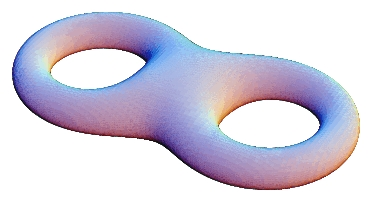
\includegraphics[width= \textwidth]{./2Torus.jpg}
\caption{An example of a two-holed torus.}
\end{figure}

Each hole allows us to encode two new qubits, since there is a way to create a series of  $Z$ or $X$ operators that cannot be deformed into each other. For a number of $n$ handles, we can encode $2n$ qubits. We call this an $n$-tori. 

This holds for any code with edges - it doesn't have to be cyclic. Consider a surface consisting of 9 plaquettes. 

\begin{figure}[h]
\centering
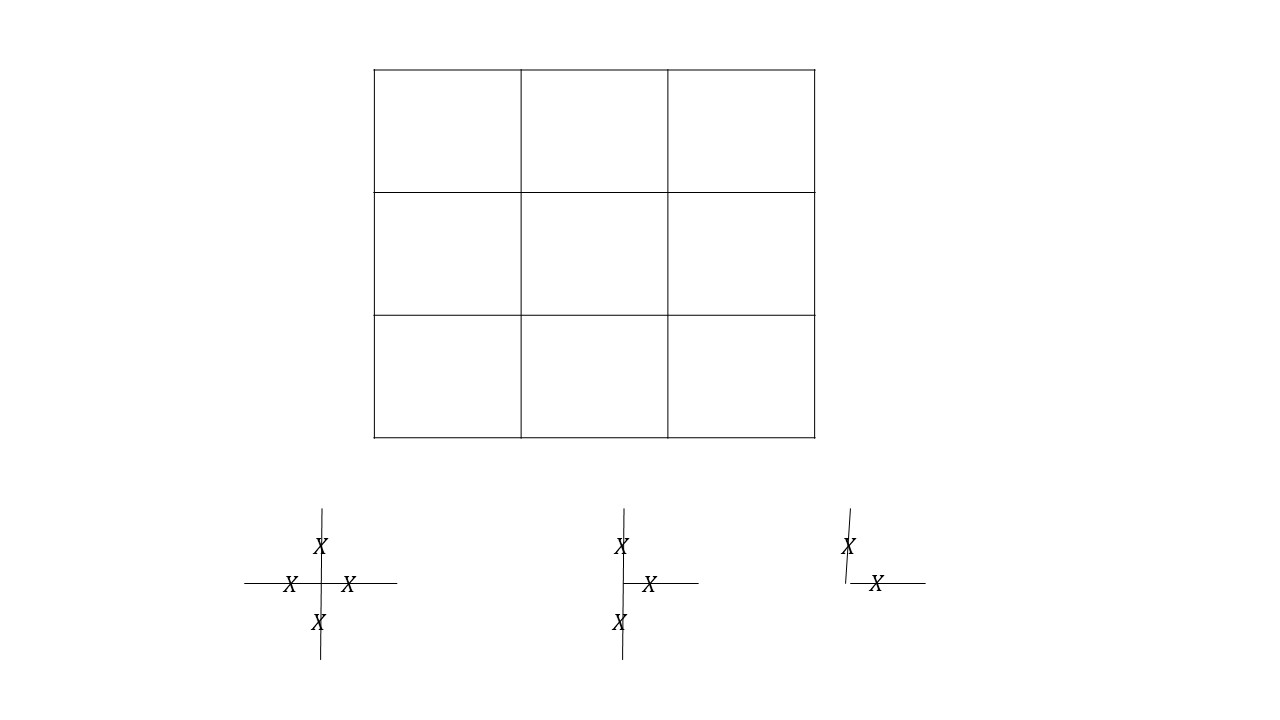
\includegraphics[width= \textwidth]{./PlanarCode.jpg}
\caption{A non-periodic code made of 9 plaquettes with three different kind of vertices.}
\end{figure}

At the edge, the surface operators have lower weight because we have to modify them to fit in with these edges. 

So, let's check how many generators we end up with $k = n-m$. Recall that $n$ is the number of physical qubits. Here, we have
\beq
2l^2 + 2l = 2l(l+1)
\eeq
So, for $l = 3$, $n = 24$, which makes sense. 

The number of plaquettes is $l^2 = 9$ and the number of vertices are $(l+1)^2 = 16$. So then, 
\beq
k = 24-25 = -1
\eeq
Something must have gone wrong - we must think about operator independence. It turns out that all plaquettes are independent. There is nothing that can cancel the operators on the edges. However, the vertices are \emph{not} independent. We must remove one, and then we get
\beq
k = 24 - 24 = 0
\eeq
There are no qubits encoded here. Also, notice that the asymmetry between plaquettes and vertices means that we have no dual properties that we can take into account. 

This was however a very naive attempt. We can change the edges to recover some symmetry properties. 

In order to encode a single qubit, we need two different types of edges: smooth and rough. 


\begin{figure}[h]
\centering
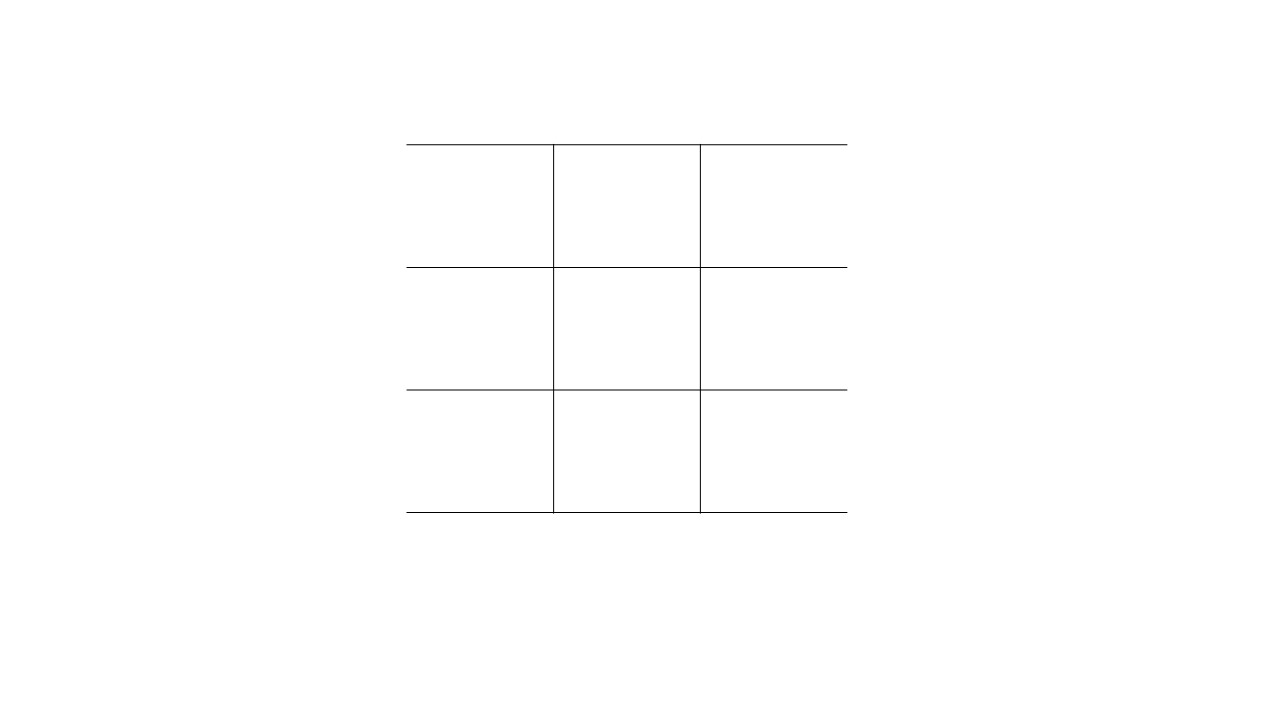
\includegraphics[width= \textwidth]{./Borders.jpg}
\caption{An example of a code with rough edges left and right, and smooth edges on the top and the bottom. .}
\end{figure}

Note that one of the vertices, the one with only two $X$ operators disappears. Now, we can count the generators again. We find
\beq
k = 18-17 = 1
\eeq
We can encode one logical qubit in this code. All the sets that we counted are independent. So in general, ir we have two smooth and two rough edges, we encode one logical qubit. 

Then, what are the uncorrectable errors? We have, for example the logical $\bar{Z}$ and logical $\bar{X}$. The $\bar{Z}$ operator runs between rough edges, and the $\bar{X}$ operator runs between smooth edges (this might be incorrect, check it!) 


It turns out that any path between two edges is topologically equivalent. However, we are not allowed to touch the corners. They have special properties which we shall not go into here. Furthermore all the analysis that we performed for the Toric code applies here too. 

Then what about errors? A single error on the edge will get only one negative measurement by one of the plaquette or vertices. However, we can modify our error matching algorithm to take into account the boundaries. We allow the matching to associate certain vertices to the boundaries. 

The threshold are approximately the same as for the Toric code. As $L \rightarrow \infty$, it turns out that we won't have any weird side effects. 

\section{The Repetition Code}
Let us have a final look at the repetition code. We have looked at errors on most things, such as measurement and preparation, but what about errors on detection? What if our stabilisers are wrong? 

Consider a code with five physical qubits in a line. Let us put an error on the edge, but what happens then if our stabiliser is wrong and either fails to detect the error or gives us a false positive somewhere else? 

By considering the \textbf{change} in errors throughout the code as a function of time, we can avoid these mistakes through repeated measurements. The key ideas is that instead of recording the detection of an error, we will record the change from $+1 \rightarrow -1$ in a stabiliser measurement, or vice versa. 

\begin{figure}[h]
\centering
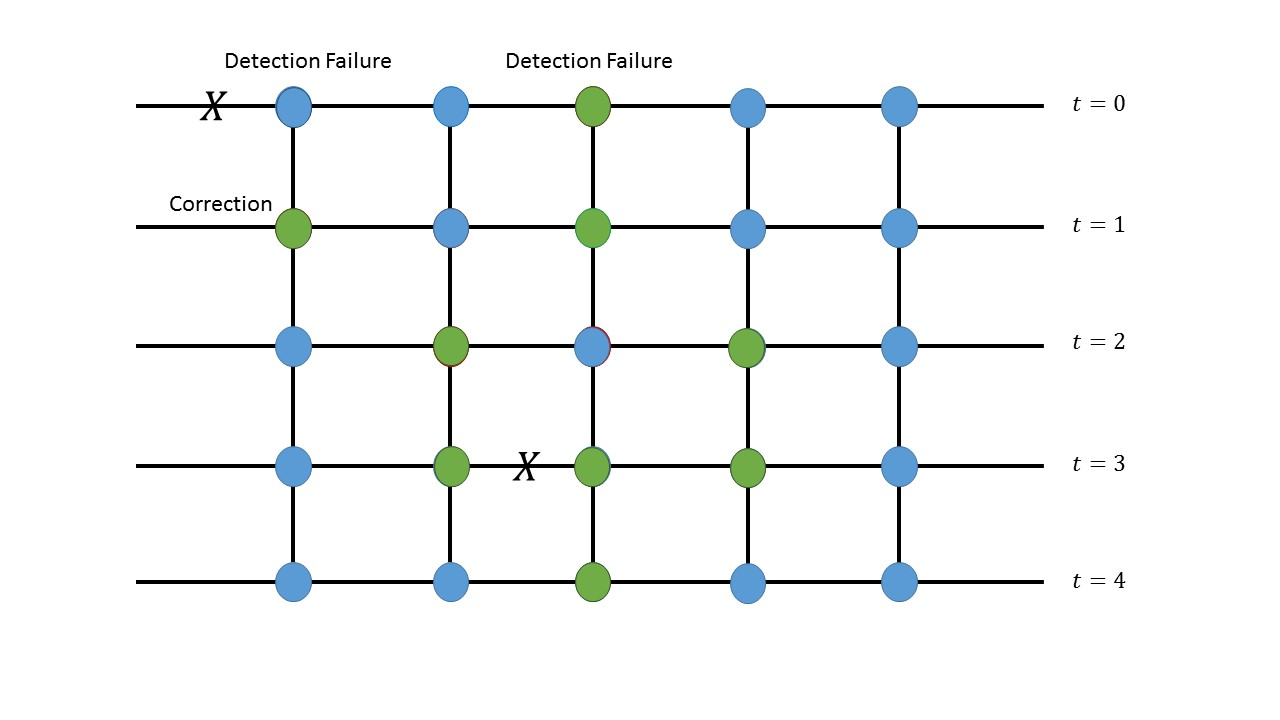
\includegraphics[width = \textwidth] {./TimeCorrection.jpg}
\caption{Recording the change (green) in the stabiliser measurements between runs.}
\end{figure}

Note: The figure in my notes is slightly different, but I'm not entirely sure how to set it right. The above seemed logical to me. 

The key idea is that we repeat the syndrome measurement. If we take the time edges into account, we find that each error is contained within one or more changes. 

Question: But what if I just have one single stabiliser failure? 

One way to correct errors is by changing to another Pauli frame. Instead of adapting our measurements, we adapt the lattice that the errors lie on. We can perform certain operations, for example, we can change the code for operations performed at later stages. This is where it gets quite technical, so we will not go further into it. Important is that we would get thresholds of about $3\%$. A gate error model (where the gates have errors that occur with probability $p$) gets a threshold of about $\mathcal{O}(0.5\% \sim 1 \%)$. This is actually quite decent. 

\section{Fault tolerant gates in the planar code}
This holds for the CSS code. The CNOT gate is transverse for all CSS codes. We have two ode blocks alongside each other and the CNOT gate acts between them. 

Implementing the Hadamard gate can be a bit tricky. We can get fault tolerant Hadamards by applying the single qubit  $H$ to each qubit and then rotating the entire code by 90 degrees. It turns out that a 90 degree rotation is equivalent to shirting the primal lattice into the dual lattice. That is, we get $Z \rightarrow X$. But on the dual, we have $X \rightarrow Z$, so we are good. We get a sequence of \textbf{code deformations}. This is not the most efficient way to implement the Hadamard, but it is fault tolerant. 

\section{more qubits}
How can we create more qubits in the planar code? We can add more holes to the lattice. We can have either smooth holes (holes with only smooth edges) and rough holes. Then, the logical qubits are any loop that goes from smooth-smooth or rough-rough. If we have a hole with only rough edges, the $\bar{Z}$ goes around the hole. 

Because we cannot deform a $Z$ gate into an $X$ gate, we can identify any loop between or around the holes. 

The code distance for $\bar{X}$ thus becomes the shortest distance between the holes. The minimum weight of $\bar{Z}$ becomes the shortest circumference around the holes. Each pair of holes can represent qubits. We have logical operators going between them as well. 

\section{Code deformation}
We are able to create holes, enlarge them or shrink them while performing the computation. We can do so by experimentally turning off one plaquette of stabilisers. Turning off is equivalent to measuring a qubit - we know its value and then cease to interact with it. 

We can enlarge a hole by turning off more plaquettes. This entire formalism relies heavily on being able to picture various transformations. Since it is quite picture heavy, we will not details it here. We will just mention that many gates can be implemented by moving holes around and manipulating the way logical operators travel around them. 



\end{document}